%Siendo el objetivo del maestro pokem\'on ganar todos los gimnasios recorriendo la menor distancia posible definimos como posible solución a una secuencia de lugares (gimnasios o pokeparadas) en donde sea posible pasar de un lugar al siguiente bajo las restricciones impuestas en el problema. La solución buscada propiamente dicho es aquella que forme el camino de menor longitud dentro de todas las soluciones posibles halladas.


%Para esto se desarrollo un algoritmo del tipo Greedy para obtener el camino de menor distancia posible. Se desarrollaron disversas podas que enunciaremos a continuaci\'on:

%\begin{itemize}
%\item Si la suma de pociones de todas las pokeparadas es inferior a la suma de pociones necesarias para derrotar a todos los gimnasios, entonces no hay solución.
%\item No se pueden repetir lugares ya visitados: ésta es una restricción por consigna.
%\item No se puede visitar un gimnasio sin la cantidad necesaria de pociones: de no contemplar esta poda se analizan caminos donde se pierde en gimnasios, los cuales por la primera restricci\'on, quedan como perdidos, y no generan solución.
%\item No se recorren pokeparadas si la mochila está llena: el objetivo de una pokeparada es rellenar la mochila de pociones. Al estar llena la mochila se desperdicia la pokeparada ya que no se la podrá volver a visitar. En adición, visitar una pokeparada innecesariamente, aumenta obligatoriamente la distancia recorrida por el maestro pokem\'on, ya que en vez de estar tomando un camino directo entre 2 lugares, accede a la pokeparada, aumentando as\'i la distancia euclidea.
%\item Si algún gimnasio requiere mayor cantidad de pociones que las que caben en la mochila, entonces no hay solución. 
%\end{itemize}

El problema propuesto plantea encontrar el menor camino a recorrer. En base a esto se decide buscar en cada paso el menor camino que una a dos puntos, generando una aproximación de heur\'istica golosa.

Para generar la heur\'istica se toma de base la lógica restrictiva de las podas del backtracking, lo que nos asegurará que de encontrar una solución será correcta. Para el paso goloso se tienen en cuenta los siguientes puntos:

\begin{itemize}
\item Se prioriza ganar gimnasios, por lo tanto de poder ganar un gimnasio se procederá a hacerlo.
\item La elección de movimiento será aquella que este más proxima al lugar actual del maestro pokemon: Se busca la m\'inima distancia entre nodos. 
\item En cada iteraci\'on de b\'usqueda de un nuevo destino, primero se evaluarán los gimnasios y luego las poke-paradas: Si ya se cuenta con una cantidad suficiente de pociones para derrotar a un gimnasio entonces se procede a vencerlo.
\item Al finalizar una rama completa, es decir habiendo recorrido todos los gimnasios de haber sido posible desde una pokeparada determinada, se vuelve a correr el algoritmo desde otra pokeparada diferente, intentando generar así una mejor solución. De encontrarla se la tomará como la mejor solución hasta el momento.
\end{itemize}
 

%Luego de lo comentado, nuestro algoritmo realiza lo siguiente:
%Inicialmente, chequea si es posible iniciar desde un gimnasio que no necesite pociones para ser derrotado, de ser as\'i iniciar\'a su camino a partir de la posici\'on donde se encuentra dicho gimnasio. En caso de que no exista un gimnasio con valor 0, nuestro algoritmo crear\'a una cantidad puntual de ramas igual a la cantidad de poke-paradas recibidas como par\'ametro para probar desde que pokeparada se obtiene el camino m\'as corto, por que estar\'a asumiendo que no existe ning\'un gimnasio que pueda ser vencido con 0 pociones.

%Por consiguiente, luego de pasar por una pokeparada, se chequear\'a si existe alg\'un gimnasio con menor cantidad de pociones que las que se tienen hasta el momento, y en caso de existir m\'as de uno se fijar\'a cual es el que se encuentra m\'as cercano a \'el e ir\'a a vencerlo. Luego de esta batalla y haber vencido el gimnasio, se vuelve a chequear si existe otro gimnasio con menor cantidad de pociones de las que nos quedan despues de la batalla anterior, si existe se ir\'a a vencer a dicho gimnasio, y en caso contrario se buscar\'a la pokeparada m\'as cercana para ir a recuperar pociones. Esta secuencia ser\'a repetida hasta ganar en todos los gimnasios y as\'i convertirse en \textbf{Maestro Pokem\'on}.

La aproximación a travez de una heurística nos permite obtener soluciones en forma mucho más rápida que el método de backtracking. El paso goloso nos permite ahorrar evaluaciones de casos en que es trivial su invalidez. Un ejemplo de una solución correcta alcanzada por el algoritmo es el siguiente:

\vspace*{0.3cm} \vspace*{0.3cm}
  \begin{center}
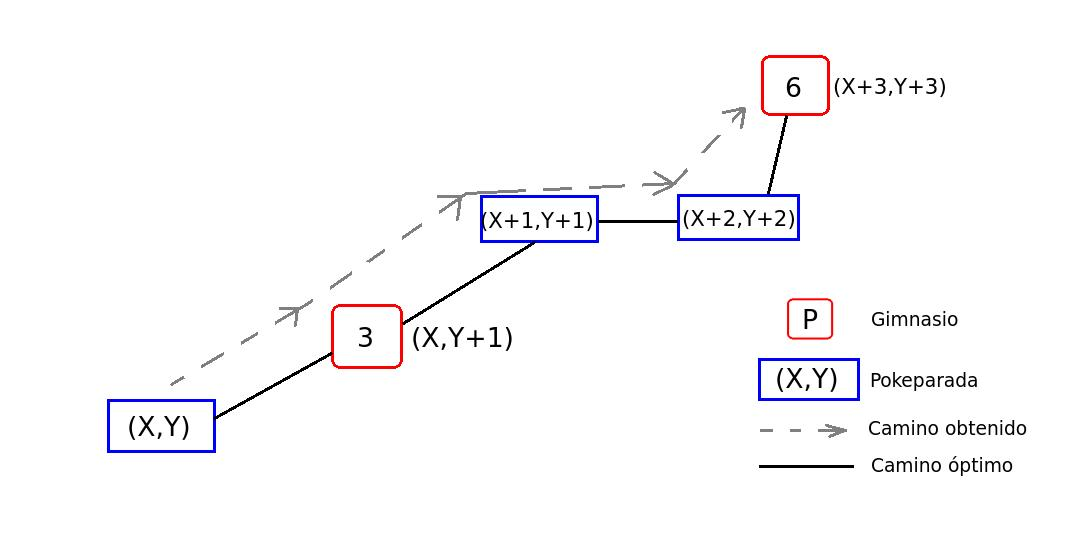
\includegraphics[scale=0.60]{./EJ2/optima.jpeg}
\\{\textit{La soluci\'on obtenida es la \'optima}}
  \end{center}
  \vspace*{0.3cm}

No obstante, la aproximación golosa tiene como desventaja de que ya no asegura que la solución a obtener sea la óptima: un ejemplo de esto se puede ver en el siguiente escenario:

\vspace*{0.3cm} \vspace*{0.3cm}
  \begin{center}
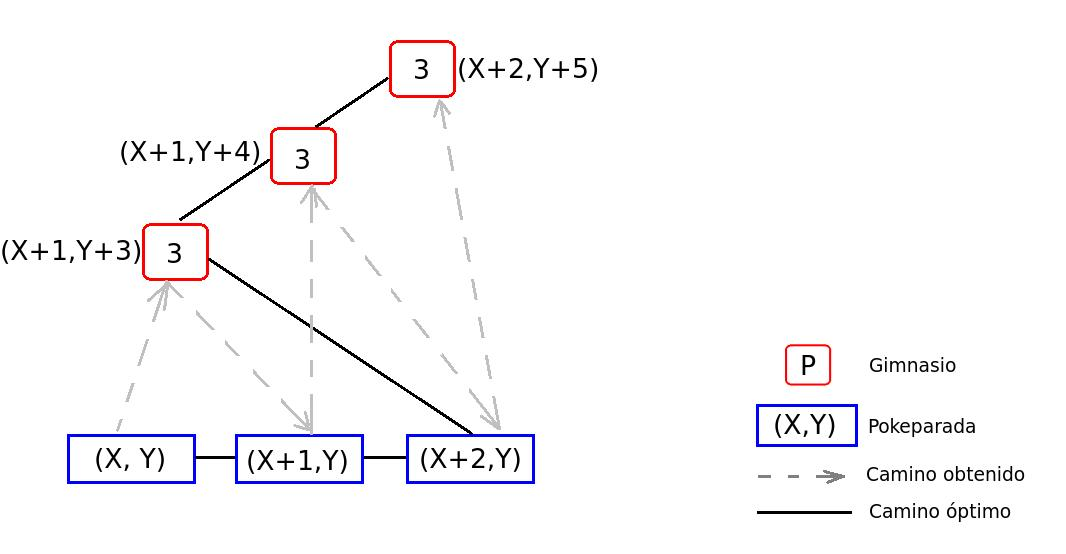
\includegraphics[scale=0.60]{./EJ2/nooptima.jpeg}
\\{\textit{La soluci\'on obtenida no es la \'optima}}
  \end{center}
  \vspace*{0.3cm}